\documentclass[11pt, spanish, letterpage]{article} %tipo de documento

\usepackage[letterpaper]{geometry} %margenes 
\geometry{verbose,tmargin=2.5cm,bmargin=2.5cm,lmargin=2cm,rmargin=2cm}
\usepackage{amsmath,amsthm,amssymb} %modos matemáticos y  simbolos
\usepackage{latexsym,amsfonts} %simbolos matematicos
\usepackage{cancel} %hacer la linea que cancela las ecuaciones
\usepackage[spanish, es-noshorthands]{babel} %comandos en español y cambia el cuadro por la tabla
\decimalpoint %cambia las comas por puntos decimal
\usepackage[utf8]{inputenc} %caracteristicas del español
\usepackage{physics} %Simbolos fisicos
\usepackage{array} %mejores formatos de tabla
\parindent =0cm %sangria 
\usepackage{graphicx} %graficas e imagenes
\usepackage{mathtools} 
\usepackage[framemethod=TikZ]{mdframed}%Entornos talegas
\usepackage[colorlinks = true,
			linkcolor = blue,
			citecolor = black,
			urlcolor = blue]{hyperref}%formato de los links y URL's
\usepackage{multicol} %varias columnas
\usepackage{enumerate} %enumeraciones
\usepackage{pgf,tikz,pgfplots} %documentos en formato tikz
\usepackage{mathrsfs} %letras chingonas (transformada de laplace)
\usepackage{subfigure} %varias figuras seguidas
\usepackage[square,numbers]{natbib} %bibliografias
\usepackage[nottoc]{tocbibind}
\bibliographystyle{plainnat}
\usetikzlibrary{arrows, babel, calc}
\usepackage{tabulary}
\usepackage{multirow} %ocupar varias filas en una tabla
\usepackage{fancybox} %recuadros talegas
\usepackage{float} %ubicar graficas
\usepackage{color}
\usepackage{comment}
\usepackage{stackrel}
\usepackage{calligra}
\usepackage{lipsum}
\usepackage{cite}
%\usepackage{showframe}
%%%%%%%%%%%%%%%%%%%%%%%%%%%%%%%%%%%%%%%%%%%%%%%%%%%%%%%%%%%
%\setlength{\columnseprule}{1pt}
%%%%%%%%%%%%%%%%%%%%%%%%%%%%%%%%%%%%%%%%%%%%%%%%%%%%%%%%%%%
\usepackage{fancyhdr}%formato de pagina
\pagestyle{fancy}%colocar la pagina con el formato deseado
\fancyhead{}
\fancyhead[L]{\footnotesize{Olimpiadas de Física Noveno}}
\fancyhead[C]{Movimiento Parabólico}
\fancyhead[R]{\footnotesize{\thepage}}
%\fancyhead[LO,RE]{Cálculo 3}
%\fancyhead[RO,LE]{\footnotesize{\thepage}}
\fancyfoot{}
\fancyfoot[L]{Diego Sarceño}
%\fancyfoot[LO,RE]{Diego Sarceño}
%%%%%%%%%%%%%%%%%%%%%%%%%%%%%%%%%%%%%%%%%%%%%%%%%%%%%%%%%%%
%-------------------------------------------------
\newcommand{\N}{\mathbb{N}}
\newcommand{\Z}{\mathbb{Z}}
\newcommand{\Q}{\mathbb{Q}}
\newcommand{\I}{\mathbb{I}}
\newcommand{\R}{\mathbb{R}}
\newcommand{\C}{\mathbb{C}} %Conjuntos numericos
\newcommand{\F}{\mathbb{F}} %Campo Cualquiera
\newcommand{\f}{\textit{f}} %f de funcion
\newcommand{\g}{\textit{g}}
\newcolumntype{E}{>{$}c<{$}} %entorno matematico en columnas de una tabla
\newcommand{\vi}{\hat{\imath}}
\newcommand{\vj}{\hat{\jmath}}%vectores unitarios R3
\newcommand\numberthis{\addtocounter{equation}{1}\tag{\theequation}}
\newcommand{\LI}{\lim _{h\longrightarrow 0}}
\newcommand{\SU}{\longrightarrow \sum _{n=0} ^{\infty}}
\newcommand{\QED}{\hfill {\qed}}
%----------------------------------------------------------
\newcommand{\Ev}{\mathbf{E}}
\newcommand{\rv}{\mathbf{r}}
\newcommand{\ru}{\hat{\rv}}
\newcommand{\zu}{\hat{\mathbf{z}}}
%----------------------------------------------------------
  
  
%-paquete para unidades en el sistema internacional
\usepackage[load=prefix, load=abbr, load=physical]{siunitx}
\newunit{\gram}{g }%gramos
\newunit{\velocity}{ \metre / \Sec }%unidades de velocidad sistema internacional
\newunit{\acceleration}{ \metre / \Sec^2 }%unidades de aceleracion sistema internacional
\newunit{\entropy}{ \joule / \kelvin }%unidades de entropia sistema internacional
%--definiendo constantes fisicas en el SI
\newcommand{\accgravity}{9.8 \metre / \Sec^2}
%---diferencial inexacta
\newcommand{\dbar}{\mathchar'26\mkern-12mu d} 
%-------------------------END-------------------------------------
%------------------------Barra Roja-------------------------------
\tikzset{
	warningsymbol/.style={
		rectangle,draw=black,
		fill=white,scale=1,
		overlay}}
\mdfdefinestyle{warning}{%
	hidealllines=true,leftline=true,
	skipabove=12,skipbelow=12pt,
	innertopmargin=0.4em,%
	innerbottommargin=0.4em,%
	innerrightmargin=0.7em,%
	rightmargin=0.7em,%
	innerleftmargin=1.7em,%
	leftmargin=0.7em,%
	middlelinewidth=.2em,%
	linecolor=black,%
	fontcolor=black,%
	firstextra={\path let \p1=(P), \p2=(O) in ($(\x2,0)+0.5*(0,\y1)$)
										node[warningsymbol] {$\ddagger$};},%
	secondextra={\path let \p1=(P), \p2=(O) in ($(\x2,0)+0.5*(0,\y1)$)
										node[warningsymbol] {$\ddagger$};},%
	middleextra={\path let \p1=(P), \p2=(O) in ($(\x2,0)+0.5*(0,\y1)$)
										node[warningsymbol] {$\ddagger$};},%
	singleextra={\path let \p1=(P), \p2=(O) in ($(\x2,0)+0.5*(0,\y1)$)
										node[warningsymbol] {$\ddagger$};},%
}

%%%%%%%%%%%%%%%%%%%%%%%%%%%%%%%%%%% Tema - BEGIN
\newtheoremstyle{Tema}% name of the style to be used
  {0mm}% measure of space to leave above the theorem. E.g.: 3pt
  {10mm}% measure of space to leave below the theorem. E.g.: 3pt
  {}% name of font to use in the body of the theorem
  {}% measure of space to indent
  {\bfseries}% name of head font
  {\newline}% punctuation between head and body
  {30mm}% space after theorem head
  {}% Manually specify head

\theoremstyle{Tema} \newtheorem{Tema}{Tema} %%%%% Template para Temas
\theoremstyle{Tema} \newtheorem{serie}{Serie}              %%%%%  Template para Series de ejercicios
\theoremstyle{Tema} \newtheorem{ejercicio}{Ejercicio}    %%%%%  Template para Ejercicios
\theoremstyle{Tema} \newtheorem{preguntas}{Preguntas}    %%%%%  Template para Ejercicios
%%%%%%%%%%%%%%%%%%%%%%%%%%%%%%%%%%% Tema - END
%-------------------------END-------------------------------------
\begin{document}
%-----------------------------------------------------------------
%							Start Here
%-----------------------------------------------------------------
%-----------------------------------------------------------------

%-----------------------------------------------------------------
%							Ecabezado
%-----------------------------------------------------------------
\begin{titlepage}

\begin{tabulary}{20cm}{LLCRR}
\multirow{4}{2.3cm}{\includegraphics[scale=0.13]{/home/diego/Documents/Licenciatura/LatexBasic/ECFM.pdf}} & Universidad de San Carlos de Guatemala  & & & \multirow{4}{4.5cm}{\hfill \includegraphics[scale=0.082]{/home/diego/Documents/Licenciatura/LatexBasic/USAC.pdf}}\tabularnewline
 & Escuela de Ciencias Físicas y Matemáticas & \hfill &  & \tabularnewline
 & Física 1 & \hfill ~~ &   & \tabularnewline
 & Diego Sarceño 201900109 & &  & \tabularnewline
 & \today &  & & \tabularnewline
\end{tabulary}\\[0.75cm]

{\hrule height 1.5pt} \vspace{0.1cm}
\begin{tabulary}{21cm}{p{5.5cm}p{7cm}p{8.5cm}}
    \hfill & \huge{\scshape{Tiro Parabólico}} & \hfill
\end{tabulary}
{\hrule height 1.5pt} 
\vspace{0.5cm}

%%%%%%%%%%%%%%%%%%%%%%%%%%%%%%%%%%
%Comando a recalcar \stackrel[abajo]{arrba}{objeto}
%Tipo de Letra \scshape{}
%\marginpar{}
%\dfrac{}{} es equivalente a \displaystyle\frac{}{}
%\textsuperscript{*}
%%%%%%%%%%%%%%%%%%%%%%%%%%%%%%%%%%
\textbf{Instrucciones: } Resuelva esta hoja de trabajo, resalte sus respuestas en lapicero negro o azul.

\section*{Movimiento Parabólico}
\begin{mdframed}[style=warning] % preguntas 1
    \begin{preguntas}
        Responda las siguientes preguntas.
        \begin{description}
            \item[Investigue: ] ¿Cuál es el ángulo que genera el alcance horizontal máximo, y cómo se reescribiría la ecuación de alcance horizontal?
        \end{description}
    \end{preguntas}
\end{mdframed}
\begin{mdframed}[style=warning] % Ejercicio 1
    \begin{ejercicio}
        Un libro de física que se desliza sobre una mesa horizontal a $1.10 \velocity$ cae y llega al piso en $0.350 \Sec$. Ignore la resistencia del aire.
        Calcule $a)$ la altura de la mesa con respecto al piso; $b)$ la distancia horizontal del borde de la mesa al punto donde cae el libro.
    \end{ejercicio}
\end{mdframed}


\begin{mdframed}[style=warning] % Ejercicio 2
    \begin{ejercicio}
        Un mariscal de campo novato lanza un balón con una componente
        de velocidad inicial hacia arriba de $12.0 \velocity$ y una componente
        de velocidad horizontal de $20.0 \velocity$. Ignore la resistencia del aire.
        $a)$ ¿Cuánto tiempo tardará el balón en llegar al punto más alto de la
        trayectoria? $b)$ ¿A qué altura está este punto? $c)$ ¿Cuánto tiempo pasa
        (desde que se lanza) para que el balón vuelva a su nivel original?
        ¿Cómo se compara este tiempo con el calculado en el inciso $a)$?
        $d)$ ¿Qué distancia horizontal viaja el balón en este tiempo? $e)$ Dibuje
        las gráficas x-t, y-t, vx-t y vy-t para el movimiento (dibujelas aproximadas no es necesario que las dibuje exactas).
    \end{ejercicio}
\end{mdframed}
\begin{mdframed}[style=warning] % Ejercicio 3
    \begin{ejercicio}
        Dentro de una nave espacial en reposo sobre la Tierra, una
        pelota rueda desde la parte superior de una mesa horizontal y cae
        al piso a una distancia $D$ de la pata de la mesa. Esta nave espacial
        ahora desciende en el inexplorado planeta $X$. El comandante, el Capitán
        Curioso, hace rodar la misma pelota desde la misma mesa con la
        misma rapidez inicial que en la Tierra, y se da cuenta de que la pelota
        cae al piso a una distancia de $2.76D$ de la pata de la mesa. ¿Cuál es
        la aceleración debida a la gravedad en el planeta $X$?
    \end{ejercicio}
\end{mdframed}
\begin{mdframed}[style=warning] % Ejercicio 4
    \begin{ejercicio}
        Gane el premio. En una feria, se puede ganar una jirafa de
        peluche lanzando una moneda a un platito, el cual está sobre una repisa
        más arriba del punto en que la moneda sale de la mano y a una distancia
        horizontal de $2.1 \metre$ desde ese punto. Si usted lanza
        la moneda con velocidad de $6.4\velocity$, a un ángulo de $60^o$ sobre la horizontal,
        la moneda caerá en el platito. Ignore la resistencia del aire. $a)$ ¿A qué altura está la repisa sobre el punto donde se lanza la moneda?
        $b)$ ¿Qué componente vertical tiene la velocidad de la moneda justo
        antes de caer en el platito?
        \begin{figure}[H]
            \centering
            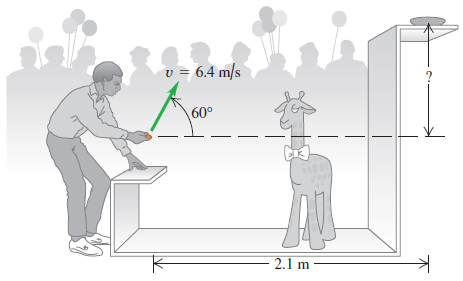
\includegraphics[scale=0.6]{JIRAFA.PNG}
            \caption{Ejercicio 4}
            \label{JIRAFA}
        \end{figure}
    \end{ejercicio}
\end{mdframed}
\begin{mdframed}[style=warning] % Ejercicio 5
    \begin{ejercicio}
        Un proyectil se dispara en tal forma que su alcance horizontal es igual a tres veces su altura máxima . ¿Cuál es el ángulo de disparo?
    \end{ejercicio}
\end{mdframed}
\begin{mdframed}[style=warning] % Ejercicio 1
    \begin{ejercicio}
        Demuestre que para tener el mismo alcance horizontal en un tiro parabólico, los ángulos de salida deben ser complementarios. (El tiro parabólico cumple con la siguiente condición: $y_o = y_f$)
    \end{ejercicio}
\end{mdframed}



\end{titlepage}
\end{document}
